% ---------------------------------------------------------------- 04-robustness.tex
\section{Robustness}\label{sec:robust}

\subsection{Parameter sensitivity}\label{sec:sens}

Figure~\ref{fig:sens} varies one parameter at a time. A higher tax rate raises the shield per unit of debt but also reduces weak-state cash, so the debt limit falls: $\Dstar = 46.0$, 44.4 and 39.3 at $\tauc = 17\%$, 20\% and 30\%. A wider spread between the states, holding mean EBIT at 90, has the same effect ($\Dstar = 51.9$, 44.4 and 37.0). The value 44.4 is therefore a property of our parameters rather than a general rule. In every case, however, the limit is set by what the weak state can repay, and the gain below it is small, between 1.0\% and 1.9\% of $\VU$.

The distress cost does not move $\Dstar$; it determines how far value falls beyond it ($-0.3$, $-3.6$ and $-8.1$ at $D = 45$ for $c = 5\%$, 20\% and 40\%). There is one qualification. If $c$ is below about 3.6\%, the additional shield outweighs the distress cost even beyond the limit, so debt just above $\Dstar$ still adds value; at $c = 5\%$ the gain turns negative at $\Dstar$ but becomes positive again for $D$ above 61.5, because the defaulting weak state still deducts its full interest, which it never pays (Section~\ref{sec:model}), an artefact we do not interpret. The conclusion that debt beyond the limit destroys value therefore requires distress costs that are not negligible, consistent with the empirical estimates cited in Section~\ref{sec:intro}.

\begin{figure}[htbp]\centering
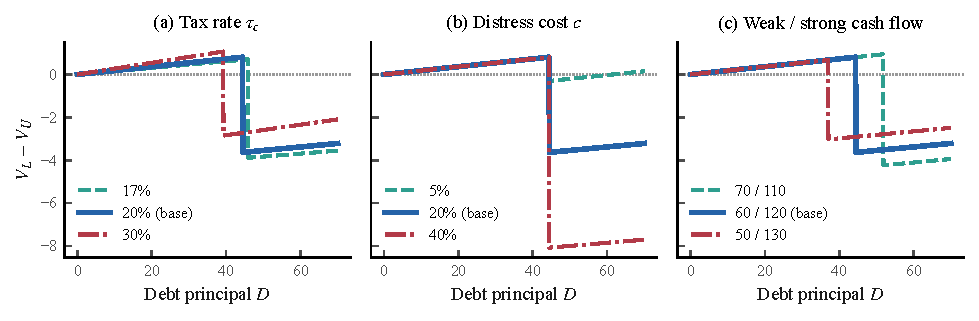
\includegraphics[width=14.2cm]{fig2_sensitivity}
\caption{Sensitivity of the two-state model to one parameter at a time. The thick solid line is the base case. In panel (c) mean EBIT is held at 90.}\label{fig:sens}
\end{figure}

\subsection{Continuous cash flows}\label{sec:cont}

The vertical drop in Figure~\ref{fig:value}a is an artefact of having only two states. With a lognormal cash flow of the same mean (standard deviation 25) and every other assumption unchanged, the value function becomes smooth and concave, the familiar trade-off between tax shield and expected distress cost \citep{kraus1973}. The optimum is near $D = 34$, where the default probability is about 1\% and the gain is 0.56, or 0.85\% of $\VU$; the gain returns to zero at $D \approx 45.5$ (Figure~\ref{fig:value}b--c). With a standard deviation of 30, which matches the dispersion of the two-state model, the optimum is near $D = 30$ with a gain of 0.49.

Both conditions are met. With $\tauc = 0$ the gain is exactly zero up to the debt limit in the two-state model and never positive in the lognormal model, and every specification produces a positive gain followed by a limit, provided distress destroys more than a few per cent of default-state cash (3.6\% in the base case).
